\documentclass[10pt]{beamer}\usepackage[]{graphicx}\usepackage{xcolor}
%% maxwidth is the original width if it is less than linewidth
%% otherwise use linewidth (to make sure the graphics do not exceed the margin)
\makeatletter
\def\maxwidth{ %
  \ifdim\Gin@nat@width>\linewidth
    \linewidth
  \else
    \Gin@nat@width
  \fi
}
\makeatother

\definecolor{fgcolor}{rgb}{0.345, 0.345, 0.345}
\newcommand{\hlnum}[1]{\textcolor[rgb]{0.686,0.059,0.569}{#1}}%
\newcommand{\hlstr}[1]{\textcolor[rgb]{0.192,0.494,0.8}{#1}}%
\newcommand{\hlcom}[1]{\textcolor[rgb]{0.678,0.584,0.686}{\textit{#1}}}%
\newcommand{\hlopt}[1]{\textcolor[rgb]{0,0,0}{#1}}%
\newcommand{\hlstd}[1]{\textcolor[rgb]{0.345,0.345,0.345}{#1}}%
\newcommand{\hlkwa}[1]{\textcolor[rgb]{0.161,0.373,0.58}{\textbf{#1}}}%
\newcommand{\hlkwb}[1]{\textcolor[rgb]{0.69,0.353,0.396}{#1}}%
\newcommand{\hlkwc}[1]{\textcolor[rgb]{0.333,0.667,0.333}{#1}}%
\newcommand{\hlkwd}[1]{\textcolor[rgb]{0.737,0.353,0.396}{\textbf{#1}}}%
\let\hlipl\hlkwb

\usepackage{framed}
\makeatletter
\newenvironment{kframe}{%
 \def\at@end@of@kframe{}%
 \ifinner\ifhmode%
  \def\at@end@of@kframe{\end{minipage}}%
  \begin{minipage}{\columnwidth}%
 \fi\fi%
 \def\FrameCommand##1{\hskip\@totalleftmargin \hskip-\fboxsep
 \colorbox{shadecolor}{##1}\hskip-\fboxsep
     % There is no \\@totalrightmargin, so:
     \hskip-\linewidth \hskip-\@totalleftmargin \hskip\columnwidth}%
 \MakeFramed {\advance\hsize-\width
   \@totalleftmargin\z@ \linewidth\hsize
   \@setminipage}}%
 {\par\unskip\endMakeFramed%
 \at@end@of@kframe}
\makeatother

\definecolor{shadecolor}{rgb}{.97, .97, .97}
\definecolor{messagecolor}{rgb}{0, 0, 0}
\definecolor{warningcolor}{rgb}{1, 0, 1}
\definecolor{errorcolor}{rgb}{1, 0, 0}
\newenvironment{knitrout}{}{} % an empty environment to be redefined in TeX

\usepackage{alltt}

\usepackage[english]{babel}
\usepackage[T1]{fontenc}
\usepackage[utf8]{inputenc}
\usepackage{amsmath}
\usepackage{array}
\usepackage{adjustbox}
\usepackage{xspace}
\usepackage{tikz}
\usetikzlibrary{shapes,arrows,backgrounds,fit,positioning,chains,shadows,decorations.pathmorphing,decorations.pathreplacing,matrix}
\usepackage{csquotes}
\usepackage{booktabs}
\usepackage{wasysym}
\usepackage[binary-units=true]{siunitx}
\usepackage{xcolor}
\usepackage{pifont}
\usepackage{dsfont}

\definecolor{tugreen}{cmyk}{0.57, 0, 1.00, 0}
\definecolor{tugreen1}{cmyk}{0.57, 0, 1.00, 0}
\definecolor{tugreen2}{HTML}{667E4D}
\definecolor{tugreen3}{HTML}{72A544}
\definecolor{tugreen4}{HTML}{3A472E}

\usecolortheme{dove}
\usetheme{boxes}
\usefonttheme{structuresmallcapsserif}
\newenvironment{whiteframe}
{
 \usebackgroundtemplate{}
 \begin{frame}
}
{
 \end{frame}
}

\usetikzlibrary{shapes,matrix,positioning,chains,arrows,shadows,decorations.pathmorphing,fit,backgrounds}
\setbeamercolor{itemize item}{fg=tugreen1}
\setbeamercolor{itemize subitem}{fg=tugreen1}
\setbeamertemplate{itemize item}[square]
\setbeamertemplate{footline}[frame number]
\beamertemplatenavigationsymbolsempty

\title{Machine Learning in R: Package \texttt{mlr}}
\logo{
\includegraphics[scale=0.05]{mlr}}
\author{Bernd~Bischl\\ Computational Statistics, LMU}
\titlegraphic{
\includegraphics[height=.3\textheight]{mlr}}
\date{}

\newcommand{\norm}[2][\relax]{\ifx#1\relax\ensuremath{\left\Vert#2\right\Vert}\else\ensuremath{\left\Vert#2\right\Vert_{#1}}\fi}
\newcommand{\ind}{\mathds{1}}
\newcommand{\pred}[1]{\ind\left(#1\right)}
\newcommand{\abs}[1]{\ensuremath{\left| #1 \right|}}
\newcommand{\code}[1]{\texttt{#1}}
\newcommand{\pkg}[1]{\texttt{#1}}
\newcommand{\tarrow}{\textcolor{tugreen1}{{\ding{212}}}\xspace}

% suppress frame numbering, so noframenumbering works
% \setbeamertemplate{frametitle continuation}
%   \begin{frame}[containsverbatim,allowframebreaks,noframenumbering]

\newenvironment{vframe}
{
  \begin{frame}[containsverbatim]
}
{
 \end{frame}
}

\newenvironment{vbframe}
{
  \begin{frame}[containsverbatim,allowframebreaks]
}
{
 \end{frame}
}

\newenvironment{blocki*}
{
  \begin{block}{}\begin{itemize}
}
{
\end{itemize}\end{block}
}

\newenvironment{blocki}[1]
{
  \begin{block}{#1}\begin{itemize}
}
{
\end{itemize}\end{block}
}

\newcommand{\oneliner}[1]{\begin{block}{}\begin{center}\begin{Large}#1\end{Large}\end{center}\end{block}}


\renewcommand<>{\sout}[1]{
  \only#2{\beameroriginal{\sout}{#1}}
  \invisible#2{#1}
}


\AtBeginSection{\frame{\sectionpage}}
\IfFileExists{upquote.sty}{\usepackage{upquote}}{}
\begin{document}
% \usebackgroundtemplate{
%   \begin{tikzpicture}
%     \shade [inner color = white, outer color = gray!30, opacity = 0.8] (\paperwidth,\paperheight) rectangle (0,0);
%     \shade [inner color = white, outer color = gray!10, opacity=.05] (\paperwidth/2,\paperheight/2) circle (3);
%   \end{tikzpicture}
% }



%% PART I
\begin{frame}
  \titlepage
\end{frame}


\begin{vframe}{About}
  \begin{itemize}
    \item Project home page\\
    \oneliner{\url{https://github.com/mlr-org/mlr}}
      \begin{itemize}
        \item \textbf{Tutorial} for online viewing / download, including many examples
        \item R documentation rendered in HTML
        \item If you are interested you can ask questions in the github issue tracker
        % \item Wiki page for this tutorial (slides, hands on solutions, \ldots)
      \end{itemize}
    \item 8-10 main developers, quite a few contributors, 4 GSOC projects in 2015/16 and 
    one coming in 2017
    \item About 20K lines of code, 8K lines of unit tests
    % \item If you do not have \pkg{mlr} installed yet, please do so (see wiki page)
      % \item Same for \pkg{OpenML} (not on CRAN, you'll need \pkg{devools}):
% <<openml-install,eval=FALSE>>=
% install.packages("devtools")
% devtools::install_github("openml/r")
% @
  \end{itemize}
\end{vframe}

% \begin{vframe}{Overview}
  % \tableofcontents
% \end{vframe}

% \begin{vframe}
%   \begin{blocki}{What is (supervised) machine learning?}
%   \item Learning structure in data:\\
%     Classification, regression, survival analysis, clustering, $\ldots$
%   \item The art of predicting stuff
%   \item Model optimization
%   \item Understanding of grey-box models
%   \end{blocki}
% 
%   \begin{blocki}{Disclaimer}
%   \item The list is subjective and naively tailored to this talk
%   \item ML is based on math and statistics, we will (mainly) talk about structure, software, and practical issues here
%   \end{blocki}
% \end{vframe}



% \begin{vframe}{Supervised Classification tasks}
% <<classification-task-plot,echo=FALSE,fig.height=4>>=
% set.seed(1)
% df = data.frame(x = c(rnorm(10, mean = 3), rnorm(10, mean = 5)), y = runif(10), class = rep(c("a", "b"), each = 10))
% ggplot(df, aes(x = x, y = y, shape = class, color = class)) + geom_point(size = 3) + geom_vline(xintercept = 4, linetype = "longdash")
% @
% \structure{Goal}: Predict a class (or membership probabilities)
% \end{vframe}


% \begin{vframe}{Supervised Regression tasks}
% <<regression-task-plot,echo=FALSE,fig.height=4>>=
% set.seed(1)
% f = function(x) 0.5 * x^2 + x + sin(x)
% x = runif(40, min = -3, max = 3)
% y = f(x) + rnorm(40)
% df = data.frame(x = x, y = y)
% ggplot(df, aes(x, y)) + geom_point(size = 3) + stat_function(fun = f, color = "#FF9999", size = 2)
% @
% \structure{Goal}: Predict a continuous output
% \end{vframe}


% \begin{vframe}{Supervised Survival tasks}
% <<survial-task-plot,echo=FALSE,fig.height=4>>=
% set.seed(1)
% data("rats", package = "survival")
% sf = survfit(Surv(time, status) ~ rx, data = rats)
% survMisc:::autoplot.survfit(sf, title = "", xLab = "Time", yLab = "$\\hat{S}(t)$\n", survLineSize = 1.5)$plot
% @
% \structure{Goal}: Predict a survival function $\hat{S}(t)$, i.e.\ the probability to survive to time point~$t$
% \end{vframe}


% \begin{vframe}{Unsupervised Cluster tasks}
% <<cluster-task-plot,echo=FALSE,fig.height=4>>=
% df = iris
% m = as.matrix(cbind(df$Petal.Length, df$Petal.Width),ncol=2)
% cl = (kmeans(m,3))
% df$cluster = factor(cl$cluster)
% centers = as.data.frame(cl$centers)
% ggplot(data=df, aes(x=Petal.Length, y=Petal.Width, color=cluster )) +
%  geom_point() +
%  geom_point(data=centers, aes(x=V1,y=V2, color='Center')) +
%  geom_point(data=centers, aes(x=V1,y=V2, color='Center'), size=52, alpha=.3) +
%  theme(legend.position="none")
% @
% \structure{Goal}: Group data into similar clusters (or estimate fuzzy membership probabilities)
% \end{vframe}


% \section{Why mlr?}
\begin{vframe}{Motivation}
  \begin{blocki}{The good news}
  \item CRAN serves hundreds of packages for machine learning
    % (cf.\ CRAN task view machine learning)
  \item Often compliant to the unwritten interface definition:
\begin{knitrout}\scriptsize
\definecolor{shadecolor}{rgb}{0.969, 0.969, 0.969}\color{fgcolor}\begin{kframe}
\begin{alltt}
\hlstd{> }\hlstd{model} \hlkwb{=} \hlkwd{fit}\hlstd{(target} \hlopt{~} \hlstd{.,} \hlkwc{data} \hlstd{= train.data, ...)}
\hlstd{> }\hlstd{predictions} \hlkwb{=} \hlkwd{predict}\hlstd{(model,} \hlkwc{newdata} \hlstd{= test.data, ...)}
\end{alltt}
\end{kframe}
\end{knitrout}
\noindent   \end{blocki}
% \end{vframe}

% \begin{vframe}{Motivation}
  \begin{blocki}{The bad news}
    \item Some packages API is \enquote{just different}
    \item Functionality is always package or model-dependent, even though the procedure might be general
    \item No meta-information available or buried in docs 
      % (sometimes not documented at all)
    % \item Many packages require the user to \enquote{guess} good hyperparameters
    % \item Result: engthy, tedious and error-prone code
  \end{blocki}
  \oneliner{Our goal: A domain-specific language for many machine learning concepts!}
\end{vframe}


\begin{vframe}{Motivation: \pkg{mlr}}
  \begin{itemize}
    \item Unified interface for the basic building blocks: tasks, learners, resampling, hyperparameters, \ldots
    \item Reflections: nearly all objects are queryable (i.e.\ you can ask them for their properties and program on them)
    \item The OO-structure allows many generic algorithms:
      \begin{itemize}
        \item Bagging
        \item Stacking
        \item Feature Selection
        \item \ldots
      \end{itemize}
    \item Easily extensible via S3
      \begin{itemize}
        \item Extension is not covered here, but explained in detail in the online tutorial
        \item You do not need to understand S3 to use \pkg{mlr}
        \item Wondering why we don't use S4? We care about code bloat and speed.
      \end{itemize}
  \end{itemize}
\end{vframe}

\begin{vframe}{}
\begin{knitrout}\scriptsize
\definecolor{shadecolor}{rgb}{0.969, 0.969, 0.969}\color{fgcolor}

{\centering 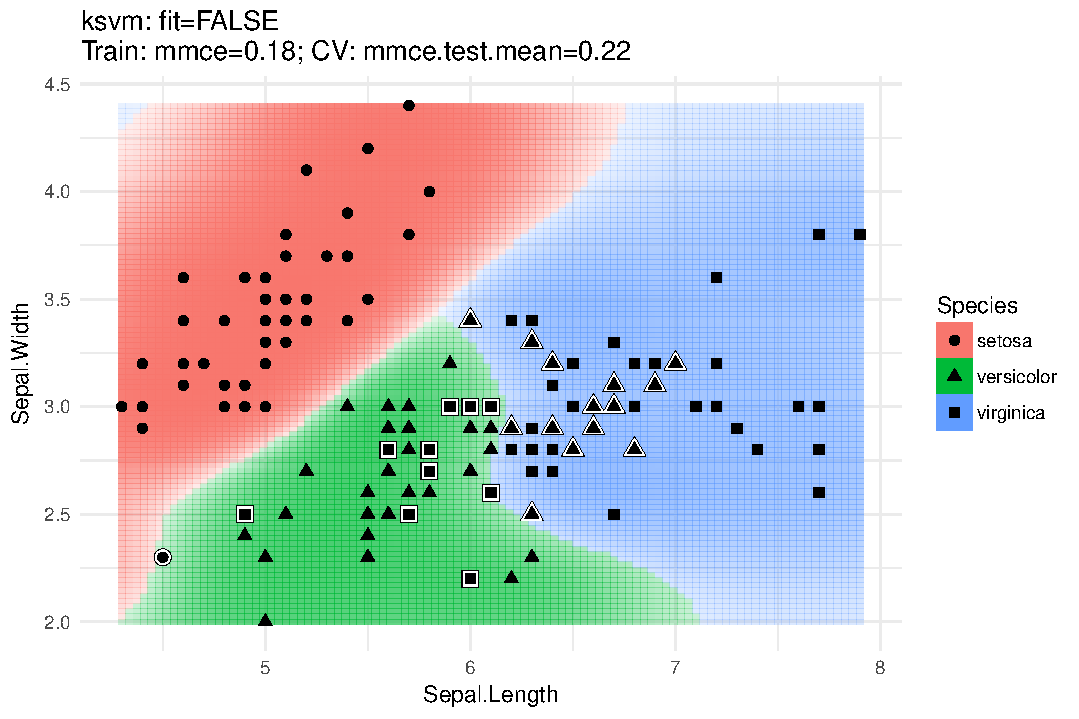
\includegraphics[width=\maxwidth]{knitr/figures/unnamed-chunk-1-1} 

}



\end{knitrout}

\noindent \end{vframe}

% \begin{vframe}{Some remarks on style}
%   \begin{blocki*}
%   \item Function names are camel-case: doThatThing()
%   \item Arguments and variables are lower-case, with dots: doThatThing(my.arg, another.one)
%   \item We use \enquote{\code{=}} not \enquote{\code{<-}}
%   \item We document in a pretty formal fashion, including type info
%   \item We try to use \enquote{@family} to group functions in the docs
%   \item We try to arg- and user-error-check in the most safe and informative way
%   \end{blocki*}
% \end{vframe}

% \section{Building Blocks}



\begin{frame}{Building Blocks}
  \begin{center}
    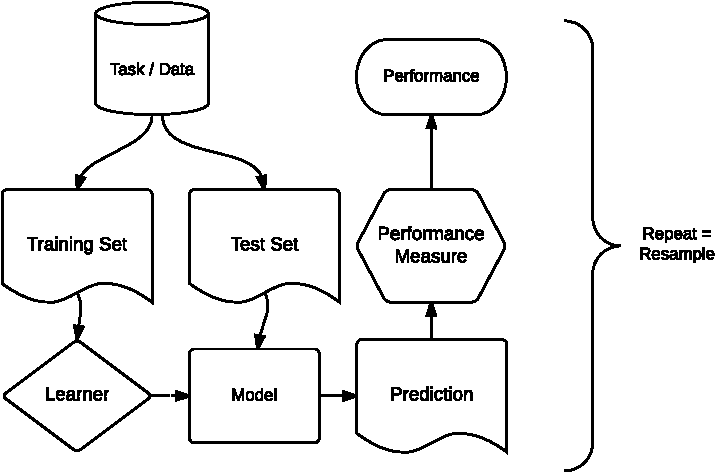
\includegraphics[width=0.9\textwidth]{figure/ml_abstraction-crop.pdf}
  \end{center}
  \begin{itemize}
    \item \pkg{mlr} objects: tasks, learners, measures, resampling instances.
  \end{itemize}
\end{frame}

% \begin{vframe}{Task Abstraction}
%   \begin{itemize}
%     \item Tasks encapsulate data and meta-information about it
%     \item Regression, classification, clustering, survival tasks
%     \item Data is stored inside an environment to save memory
%   \end{itemize}
% <<task1>>=
% task = makeClassifTask(data = iris, target = "Species")
% print(task)
% @
% \end{vframe}


% \begin{vbframe}{Task Abstraction: API}
% <<task2>>=
% getTaskId(task)
% str(getTaskData(task))
% @
% \framebreak
% <<task3>>=
% str(getTaskDescription(task))
% @
% \framebreak
% <<task4>>=
% getTaskSize(task)
% getTaskFeatureNames(task)
% getTaskTargetNames(task)
% getTaskFormula(task)
% summary(getTaskTargets(task))
% @
% \end{vbframe}


% \begin{vframe}{Learner Abstraction}
%   \begin{itemize}
%     \item Internal structure of learners:
%       \begin{itemize}
%         \item wrappers around \code{fit()} and \code{predict()} of the package
%         \item description of the parameter set
%         \item annotations
%       \end{itemize}
%     \item Naming convention: \texttt{<tasktype>.<functionname>}\\
%       e.g.: classif.svm, regr.lm
% % <<naming-convention,eval=FALSE>>=
% % makeLearner("classif.rpart")
% % makeLearner("regr.rpart")
% % @
%     % \item For the lazy: Instead of creating the object, you can also pass a string to nearly
%     %   every function that takes a learner
%     % \item Reduction algorithms for cost-sensitive classification
%     \item Adding custom learners is covered in the tutorial
%   \end{itemize}
% % \framebreak
% <<learner1>>=
% lrn = makeLearner("classif.svm", predict.type = "prob", kernel = "linear", cost = 1)
% print(lrn)
% @
% \end{vframe}

\begin{vbframe}{What Learners are available?}
  \begin{scriptsize}
  \begin{columns}
    \column{0.5\textwidth}
    \begin{blocki}{Classification (82)}
        \item LDA, QDA, RDA, MDA
        \item Trees and forests
        \item Boosting (different variants)
        \item SVMs (different variants)
        \item \ldots
    \end{blocki}
    \begin{blocki}{Clustering (9)}
        \item K-Means
        \item EM
        \item DBscan
        \item X-Means
        \item \ldots
    \end{blocki}
    \column{0.4\textwidth}
    \begin{blocki}{Regression (63)}
        \item Linear, lasso and ridge
        \item Boosting
        \item Trees and forests
        \item Gaussian processes
        \item \ldots
    \end{blocki}
    \begin{blocki}{Survival (15)}
        \item Cox-PH
        \item Cox-Boost
        \item Random survival forest
        \item Penalized regression
        \item \ldots
    \end{blocki}
  \end{columns}
  \end{scriptsize}
  \oneliner{We can explore them on the webpage -- or ask \pkg{mlr}}

\framebreak

\begin{knitrout}\scriptsize
\definecolor{shadecolor}{rgb}{0.969, 0.969, 0.969}\color{fgcolor}\begin{kframe}
\begin{alltt}
\hlstd{> }\hlcom{# list all classification learners which can predict probabilities}
\hlstd{> }\hlcom{# and allow multiclass classification}
\hlstd{> }\hlkwd{listLearners}\hlstd{(}\hlstr{"classif"}\hlstd{,}
\hlstd{+ }  \hlkwc{properties} \hlstd{=} \hlkwd{c}\hlstd{(}\hlstr{"prob"}\hlstd{,} \hlstr{"multiclass"}\hlstd{))[}\hlnum{1}\hlopt{:}\hlnum{5}\hlstd{,} \hlkwd{c}\hlstd{(}\hlopt{-}\hlnum{2}\hlstd{,} \hlopt{-}\hlnum{5}\hlstd{,} \hlopt{-}\hlnum{16}\hlstd{)]}
\end{alltt}
\begin{verbatim}
##              class short.name      package    type installed numerics
## 1   classif.avNNet     avNNet         nnet classif      TRUE     TRUE
## 2      classif.bdk        bdk      kohonen classif      TRUE     TRUE
## 3 classif.boosting     adabag adabag,rpart classif      TRUE     TRUE
## 4      classif.C50        C50          C50 classif      TRUE     TRUE
## 5  classif.cforest    cforest        party classif      TRUE     TRUE
##   factors ordered missings weights prob oneclass twoclass
## 1    TRUE   FALSE    FALSE    TRUE TRUE    FALSE     TRUE
## 2   FALSE   FALSE    FALSE   FALSE TRUE    FALSE     TRUE
## 3    TRUE   FALSE     TRUE   FALSE TRUE    FALSE     TRUE
## 4    TRUE   FALSE     TRUE    TRUE TRUE    FALSE     TRUE
## 5    TRUE    TRUE     TRUE    TRUE TRUE    FALSE     TRUE
##   class.weights featimp    se lcens rcens icens
## 1         FALSE   FALSE FALSE FALSE FALSE FALSE
## 2         FALSE   FALSE FALSE FALSE FALSE FALSE
## 3         FALSE    TRUE FALSE FALSE FALSE FALSE
## 4         FALSE   FALSE FALSE FALSE FALSE FALSE
## 5         FALSE    TRUE FALSE FALSE FALSE FALSE
\end{verbatim}
\end{kframe}
\end{knitrout}

\noindent % \framebreak

% \oneliner{Get all applicable learners for a task}
% <<listlrns2>>=
% listLearners(task)[1:5, c(-2, -5, -16)]
% @

\end{vbframe}

\begin{vframe}{Parameter Abstraction}
  \begin{itemize}
    \item Extensive meta-information for hyperparameters available:\\
      storage type, constraints, defaults, dependencies
    \item Automatically checked for feasibility
    \item You can program on parameters!
    \end{itemize}
\begin{knitrout}\tiny
\definecolor{shadecolor}{rgb}{0.969, 0.969, 0.969}\color{fgcolor}\begin{kframe}
\begin{alltt}
\hlstd{> }\hlkwd{getParamSet}\hlstd{(lrn)}
\end{alltt}
\begin{verbatim}
##                        Type  len              Def                             Constr Req Tunable Trafo
## type               discrete    - C-classification C-classification,nu-classification   -    TRUE     -
## cost                numeric    -                1                           0 to Inf   Y    TRUE     -
## nu                  numeric    -              0.5                        -Inf to Inf   Y    TRUE     -
## class.weights numericvector <NA>                -                           0 to Inf   -    TRUE     -
## kernel             discrete    -           radial   linear,polynomial,radial,sigmoid   -    TRUE     -
## degree              integer    -                3                           1 to Inf   Y    TRUE     -
## coef0               numeric    -                0                        -Inf to Inf   Y    TRUE     -
## gamma               numeric    -                -                           0 to Inf   Y    TRUE     -
## cachesize           numeric    -               40                        -Inf to Inf   -    TRUE     -
## tolerance           numeric    -            0.001                           0 to Inf   -    TRUE     -
## shrinking           logical    -             TRUE                                  -   -    TRUE     -
## cross               integer    -                0                           0 to Inf   -   FALSE     -
## fitted              logical    -             TRUE                                  -   -   FALSE     -
## scale         logicalvector <NA>             TRUE                                  -   -    TRUE     -
\end{verbatim}
\end{kframe}
\end{knitrout}
\noindent \end{vframe}

% \begin{vframe}{Learner Abstraction: API}
% <<learner2>>=
% lrn$properties
% getHyperPars(lrn)
% lrn = setHyperPars(lrn, cp = 0.3)
% lrn = setPredictType(lrn, "prob")
% lrn = setPredictThreshold(lrn, 0.7);
% @
% \end{vframe}


% \begin{vframe}{Performance Measures}
%   \begin{itemize}
%     \item Performance measures evaluate the predictions a test set and aggregate them over multiple in resampling iterations
%     \item nm["classif"]~classification, nm["regr"]~regression,  nm["cluster"]~cluster, nm["surv"]~survival
%     \item Internally: performance and aggregation function, annotations
%     \item Adding custom measures is covered in the tutorial
% \end{itemize}
% <<measure>>=
% print(mmce)
% listMeasures("classif")[1:12]
% @
% \end{vframe}

% \begin{vframe}{What measures are available?}
  % \oneliner{We can explore them on the webpage -- or ask \pkg{mlr}}
% <<measure2>>=
% listMeasures("classif")
% listMeasures(task)
% @
% \end{vframe}

% \begin{vframe}{R Example}
  % \oneliner{Training and prediction}
% \end{vframe}



% \begin{vbframe}{Resampling Abstraction}
%   \begin{itemize}
%     \item Procedure: Train, Predict, Eval, Repeat.
%     \item Aim: Estimate expected model performance.
%       \begin{itemize}
%         \item Hold-Out
%         \item Cross-validation (normal, repeated)
%         \item Bootstrap (OOB, B632, B632+)
%         \item Subsampling
%         \item Stratification
%         \item Blocking
%       \end{itemize}
%     \item Instantiate it or not (= create data split indices)
%   \end{itemize}
% 
% <<resample1>>=
% rdesc = makeResampleDesc("CV", iters = 3)
% rin = makeResampleInstance(rdesc, task = task)
% str(rin$train.inds)
% @
%   \framebreak
%   \begin{blocki}{Resampling a learner}
%     \item Measures on test (or train) sets
%     \item Returns aggregated values, predictions and some useful extra information
% <<resample2>>=
% lrn = makeLearner("classif.rpart")
% rdesc = makeResampleDesc("CV", iters = 3)
% measures = list(mmce, timetrain)
% r = resample(lrn, task, rdesc, measures = measures)
% @
% \item For the lazy
% <<resample3, eval = FALSE>>=
% r = crossval(lrn, task, iters = 3, measures = measures)
% @
%   \end{blocki}
% \framebreak
% <<resample2b>>=
% print(r)
% @
% Container object: Measures (aggregated and for each test set), predictions, models, \dots
% 
% \end{vbframe}

% \begin{vframe}{Configuring the Package}

% \begin{blocki*}
%   \item What to do when training fails? error, warn, or be quiet?\\
%     \tarrow You don't want to stop in complex loops like \code{benchmark}\\
%     \tarrow \code{FailureModel} is created that predicts NAs
%   \item Show verbose info messages?
%   \item What if parameters are not described in learner?
%   \item \code{?configureMlr} sets global flags and can be overwritten for individual learners
% \end{blocki*}
% \end{vframe}




%% PART II
% \section{Part2} %----------------------------------------------------------------------------------

%\section{Benchmarking and Model Comparison} %%%%%%%%%%%%%%%%%%%%%%%%%%%%%%%%%%%%%%%%%%%%%%%%%%%%%%%%%%%%%%%%%%%%%%

\begin{vbframe}{Benchmarking and Model Comparison}
  \begin{blocki}{Benchmarking}
    \item Comparison of multiple models on multiple data sets
    \item Aim: Find best learners for a data set or domain, learn about learner characteristics, \ldots
  \end{blocki}



\begin{knitrout}\scriptsize
\definecolor{shadecolor}{rgb}{0.969, 0.969, 0.969}\color{fgcolor}\begin{kframe}
\begin{alltt}
\hlstd{> }\hlcom{# these are predefined in mlr for toying around:}
\hlstd{> }\hlstd{tasks} \hlkwb{=} \hlkwd{list}\hlstd{(iris.task, sonar.task)}
\hlstd{> }\hlstd{learners} \hlkwb{=} \hlkwd{list}\hlstd{(}
\hlstd{+ }  \hlkwd{makeLearner}\hlstd{(}\hlstr{"classif.rpart"}\hlstd{),}
\hlstd{+ }  \hlkwd{makeLearner}\hlstd{(}\hlstr{"classif.randomForest"}\hlstd{,} \hlkwc{ntree} \hlstd{=} \hlnum{500}\hlstd{),}
\hlstd{+ }  \hlkwd{makeLearner}\hlstd{(}\hlstr{"classif.svm"}\hlstd{)}
\hlstd{+ }\hlstd{)}
\hlstd{> }
\hlstd{> }\hlstd{rdesc} \hlkwb{=} \hlkwd{makeResampleDesc}\hlstd{(}\hlstr{"CV"}\hlstd{,} \hlkwc{iters} \hlstd{=} \hlnum{3}\hlstd{)}
\hlstd{> }\hlstd{br} \hlkwb{=} \hlkwd{benchmark}\hlstd{(learners, tasks, rdesc)}
\end{alltt}
\end{kframe}
\end{knitrout}

\noindent Container object: Results, individual predictions, \dots

\framebreak

\begin{knitrout}\scriptsize
\definecolor{shadecolor}{rgb}{0.969, 0.969, 0.969}\color{fgcolor}\begin{kframe}
\begin{alltt}
\hlstd{> }\hlkwd{plotBMRBoxplots}\hlstd{(br)}
\end{alltt}
\end{kframe}

{\centering 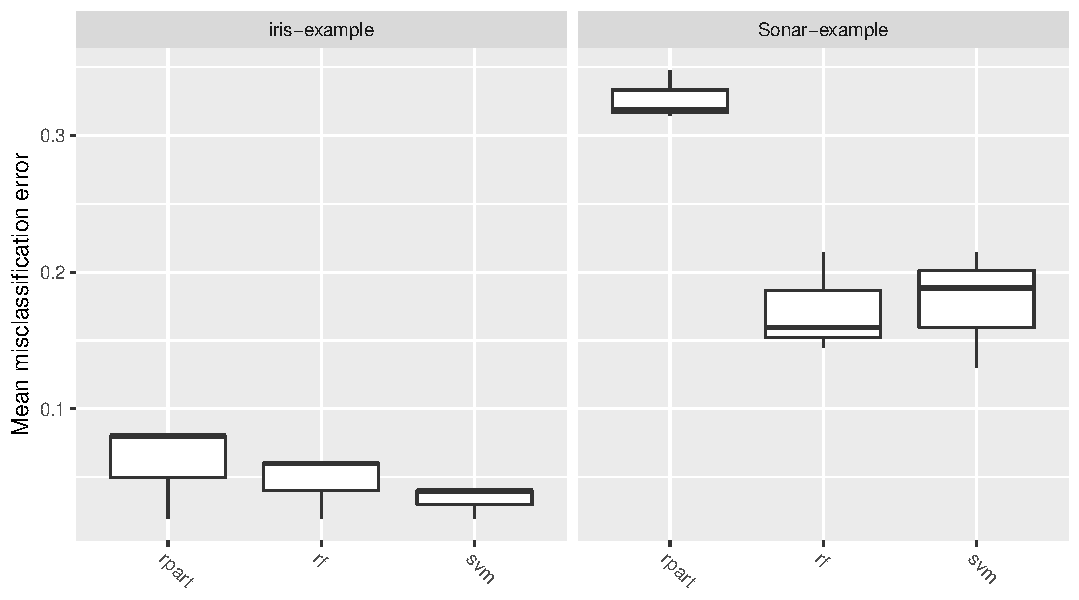
\includegraphics[width=\maxwidth]{knitr/figures/unnamed-chunk-4-1} 

}



\end{knitrout}

\noindent % \framebreak
% 
% <<eval=TRUE, fig.height=4>>=
% plotBMRRanksAsBarChart(br)
% @
% 
% \framebreak
% 
% <<warning=FALSE, fig.height=4>>=
% g = generateCritDifferencesData(br, p.value = 0.1, test = "nemenyi")
% plotCritDifferences(g) 
% @

%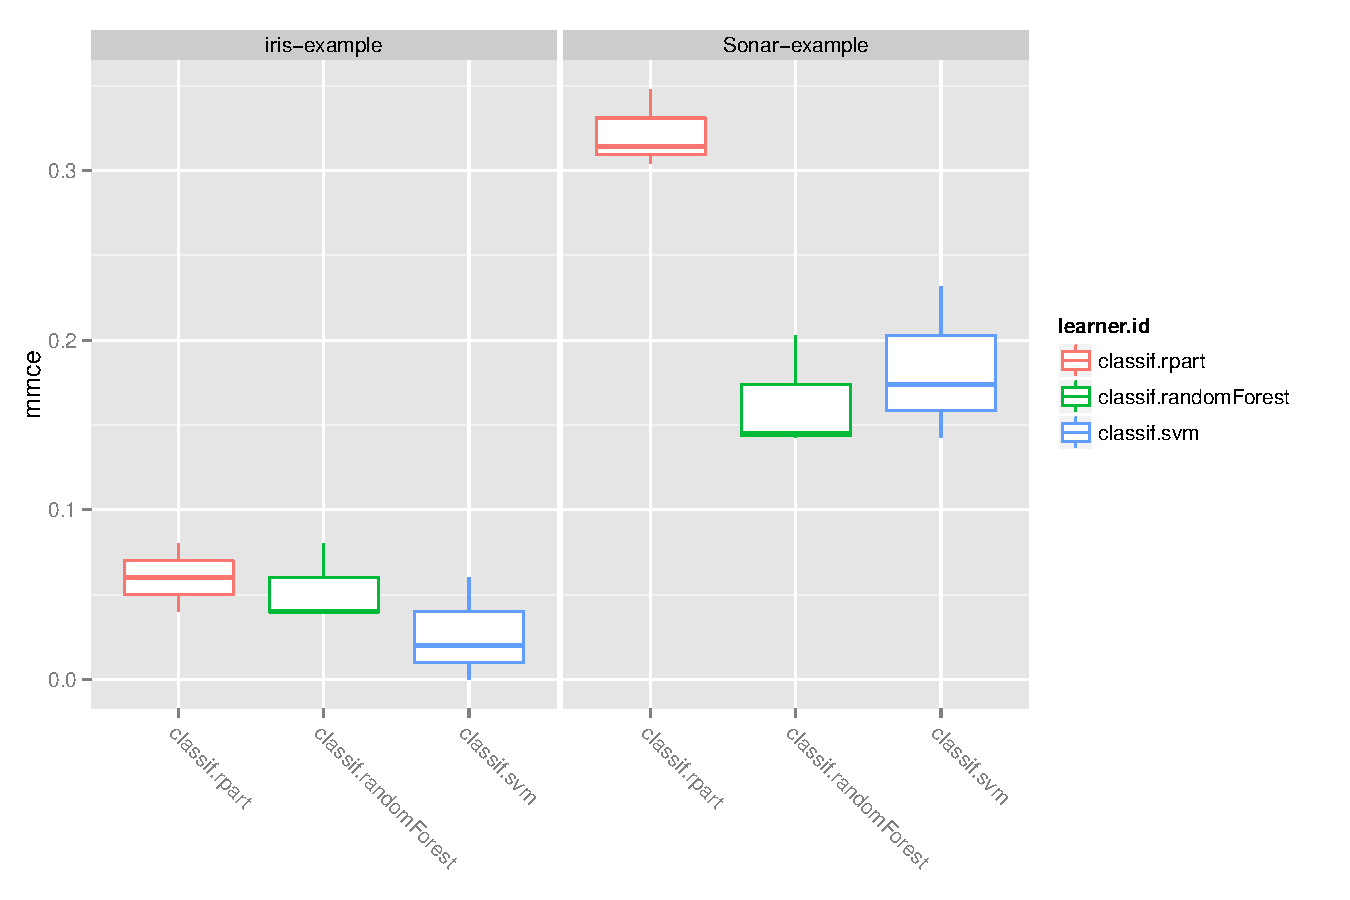
\includegraphics[width=0.9\textwidth]{figure/bmr_boxplots.pdf}

\end{vbframe}

%\section{Hyperparameter Tuning and Model Selection} %%%%%%%%%%%%%%%%%%%%%%%%%%%%%%%%%%%%%%%%%%%%%%%%%%%%%%%%%%%%%%%%%%%%%%

\begin{vframe}{Hyperparameter Tuning}
  \begin{blocki}{Tuning}
  \item Used to find \enquote{best} hyperparameters for a method in a data-dependent way
  \item General procedure: Tuner proposes param point, eval by resampling, feedback value to tuner
  \end{blocki}

  \begin{blocki}{Grid search}
  \item Basic method: Exhaustively try all combinations of finite grid\\
  $\leadsto$ Inefficient, combinatorial explosion, searches irrelevant areas
  \end{blocki}

  \begin{blocki}{Random search}
  \item Randomly draw parameters\\
  $\leadsto$ Scales better then grid search, easily extensible
  \end{blocki}
\end{vframe}


\begin{vframe}{Automatic Model Selection}
  \begin{blocki}{Prior approaches:}
  \item Looking for the silver bullet model \\
    $\leadsto$ Failure\\
  \item Exhaustive benchmarking / search \\
    $\leadsto$ Per data set: too expensive \\
    $\leadsto$ Over many: contradicting results
  \item Meta-Learning:\\
    $\leadsto$ Failure \\
    $\leadsto$ Usually not for preprocessing / hyperparamters
  \end{blocki}

  \structure{Goal}: Data dependent + Automatic + Efficient
\end{vframe}

\begin{frame}{Adaptive tuning}
  \begin{center}
    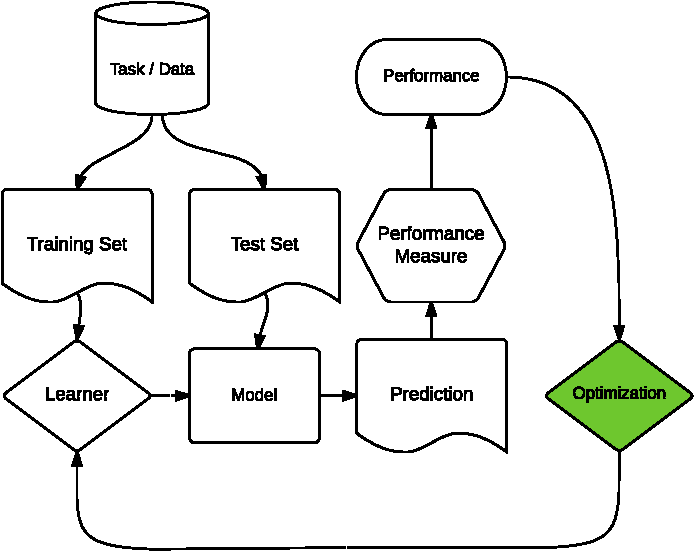
\includegraphics[width=0.85\textwidth]{figure/ml_abstraction_optimization-crop.pdf}
  \end{center}
\end{frame}

\begin{vframe}{Tuning Example}

\begin{knitrout}\scriptsize
\definecolor{shadecolor}{rgb}{0.969, 0.969, 0.969}\color{fgcolor}\begin{kframe}
\begin{alltt}
\hlstd{> }\hlstd{ps} \hlkwb{=} \hlkwd{makeParamSet}\hlstd{(}
\hlstd{+ }  \hlkwd{makeNumericParam}\hlstd{(}\hlstr{"C"}\hlstd{,} \hlkwc{lower} \hlstd{=} \hlopt{-}\hlnum{5}\hlstd{,} \hlkwc{upper} \hlstd{=} \hlnum{5}\hlstd{,} \hlkwc{trafo} \hlstd{=} \hlkwa{function}\hlstd{(}\hlkwc{x}\hlstd{)} \hlnum{2}\hlopt{^}\hlstd{x),}
\hlstd{+ }  \hlkwd{makeNumericParam}\hlstd{(}\hlstr{"sigma"}\hlstd{,} \hlkwc{lower} \hlstd{=} \hlopt{-}\hlnum{5}\hlstd{,} \hlkwc{upper} \hlstd{=} \hlnum{5}\hlstd{,} \hlkwc{trafo} \hlstd{=} \hlkwa{function}\hlstd{(}\hlkwc{x}\hlstd{)} \hlnum{2}\hlopt{^}\hlstd{x)}
\hlstd{+ }\hlstd{)}
\hlstd{> }\hlstd{ctrl} \hlkwb{=} \hlkwd{makeTuneControlRandom}\hlstd{(}\hlkwc{maxit} \hlstd{=} \hlnum{100L}\hlstd{)}
\hlstd{> }\hlstd{rdesc} \hlkwb{=} \hlkwd{makeResampleDesc}\hlstd{(}\hlstr{"CV"}\hlstd{,} \hlkwc{iters} \hlstd{=} \hlnum{2L}\hlstd{)}
\hlstd{> }\hlstd{res} \hlkwb{=} \hlkwd{tuneParams}\hlstd{(}\hlstr{"classif.ksvm"}\hlstd{,} \hlkwc{task} \hlstd{= pid.task,} \hlkwc{control} \hlstd{= ctrl,}
\hlstd{+ }  \hlkwc{resampling} \hlstd{= rdesc,} \hlkwc{par.set} \hlstd{= ps,} \hlkwc{show.info} \hlstd{=} \hlnum{FALSE}\hlstd{)}
\end{alltt}
\end{kframe}
\end{knitrout}

\noindent \begin{knitrout}\scriptsize
\definecolor{shadecolor}{rgb}{0.969, 0.969, 0.969}\color{fgcolor}

{\centering 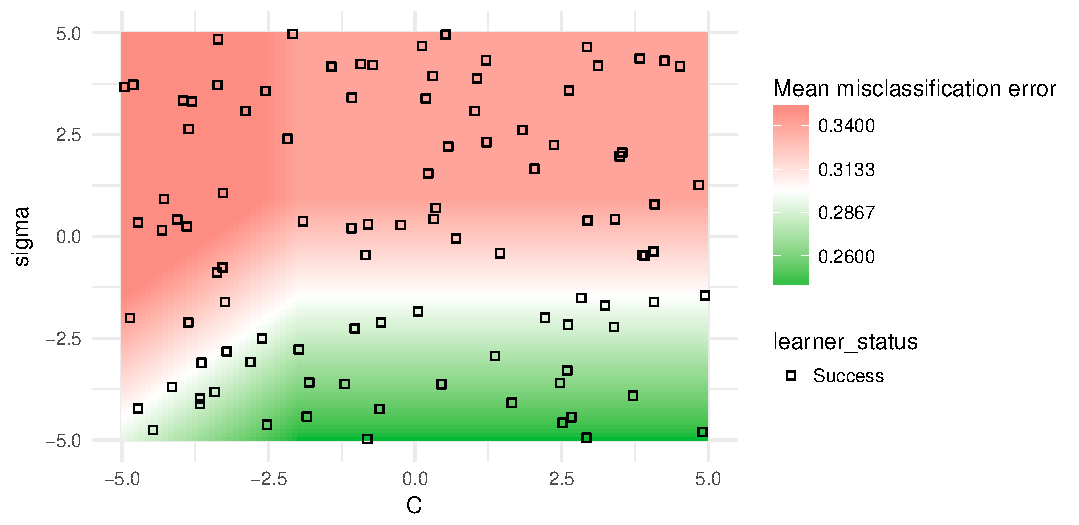
\includegraphics[width=\maxwidth]{knitr/figures/unnamed-chunk-6-1} 

}



\end{knitrout}


\noindent \end{vframe}


% \begin{vframe}{General Algorithm Configuration}
% \begin{itemize}
%   \item Assume a (parametrized) algorithm $a$
%   \item Parameter space  $\theta \in \Theta$\\
%         might be discrete and dependent / hierarchical
%   \item Stochastic generating process for instances $i \sim P$, where we draw i.i.d. from.
%         % (Usually predefined set of instances, and i.i.d.-ness somewhat violated)
%   \item Run algorithm $a$ on $i$ and measure performance $f(i, \theta) = run(i, a(\theta))$
%   \item Objective: $\min_{\theta \in \Theta} E_P[f(i, \theta)]$
%   \item No derivative for $f(\cdot, \theta)$, black-box
%   \item $f$ is stochastic / noisy
%   \item $f$ is likely expensive to evaluate
%   \item \textbf{Consequence: very hard problem}
% \end{itemize}
% $\leadsto$ \structure{\textbf{Racing or model-based / bayesian optimization}}
% % \item VERY poopular nowadays to configure, e.g., discrete solvers for NP-hard problems
% \end{vframe}
% 
% 
% \begin{frame}{Idea of (F-)Racing}
%   \begin{columns}
%     \begin{column}{.35\textwidth}
%       \begin{tikzpicture}[scale=0.18]
%         %%%%%%%%%%%%%%%%%%%%%%%%%%%%%%%%%%%%%%%%%%%%%%%%%%%%%%%%%%%%%%%%%%%%%%%%%%%%
% Author: Manuel López-Ibáñez <manuel.lopez-ibanez@ulb.ac.be>
%
% License: Copyright  Manuel López-Ibáñez
%          CC-BY-3.0 http://creativecommons.org/licenses/by/3.0/
%%%%%%%%%%%%%%%%%%%%%%%%%%%%%%%%%%%%%%%%%%%%%%%%%%%%%%%%%%%%%%%%%%%%%%%%%%

\providecommand{\raceConfigurations}{$\Theta$}

\tikzstyle{hidden} = [white,color=white];
\tikzstyle{unselected} = [black,color=black];
\tikzstyle{selected} = [green,color=green, line width=1.5pt];
\tikzstyle{discarded} = [red,color=red, line width=1.5pt];

\tikzstyle{every node}=[font=\normalsize];
\tikzstyle{every path} = [line width=1pt];
\tikzstyle{arrow1} = [black,color=black];
\tikzstyle{arrow2} = [black,color=black];

%%% Local Variables: 
%%% mode: latex
%%% TeX-master: t
%%% End: 

%         %%%-*- mode: latex; TeX-master: "race-test"-*-%
%%%%%%%%%%%%%%%%%%%%%%%%%%%%%%%%%%%%%%%%%%%%%%%%%%%%%%%%%%%%%%%%%%%%%%%%%%
% Author: Manuel López-Ibáñez <manuel.lopez-ibanez@ulb.ac.be>
%
% License: Copyright  Manuel López-Ibáñez
%          CC-BY-3.0 http://creativecommons.org/licenses/by/3.0/
%
%%%%%%%%%%%%%%%%%%%%%%%%%%%%%%%%%%%%%%%%%%%%%%%%%%%%%%%%%%%%%%%%%%%%%%%%%%%
%% FIXME: 
%%
%% * Make it more compact. Draw the points once, and then use
%% \tikstyle to hide/show/color them.
%% * Fix overfull \hbox (it is caused by \raceConfigurations).
%% * Make it more configurable:
%%    - Calculate \ystart \yend w.r.t. \rows (how to do computations in tikz?)
%%    - Define variable for circle size.
%%    - Define variable for transitions.
%%    - Define commands for labels.

%\draw[style=help lines] (0,0) grid (1,45);

\def\rows{35}
\def\ystart{34.5}
\def\yend{32.5}

\onslide*<.(17)->{
  \tikzstyle{unselected} = [selected]
}
\onslide*<.(18)>{
  \draw[fill=red,draw,red] (0,\rows) rectangle (15,21);
}

\onslide*<+>{
  \foreach \y in {0} {
    \foreach \x in {0,...,14}
    \filldraw[unselected] (0.5 + \x  , \ystart - \y) circle (0.35);
  }
}

\onslide*<+>{
\tikzstyle{arrow2} = [line width=1.5pt,red];
}
\onslide*<+>{
\tikzstyle{arrow1} = [line width=1.5pt,red];
}

\draw[arrow1,->]  (0,\rows) -- (0,0) node[very near end,above,rotate=90]{Instances};
\draw[arrow2,->]  (0,\rows) -- (16,\rows) node[midway,above]{\raceConfigurations};



\foreach \y in {0,...,2} {
  \foreach \x in {0,...,14}
  \filldraw[unselected] (0.5 + \x  , \ystart - \y) circle (0.35);
  \pause
}

\onslide*<+>{
  \foreach \y in {0,...,2} {
    \foreach \x in {0,...,10}
    \filldraw[selected] (0.5 + \x  , \ystart - \y) circle (0.35);
    \foreach \x in {11,...,14}
    \filldraw[discarded] (0.5 + \x  , \ystart - \y) circle (0.35);
  }
}

\onslide*<+->{
  \foreach \y in {0,...,2} {
    \foreach \x in {0,...,14}
    \filldraw[unselected] (0.5 + \x  , \ystart - \y) circle (0.35);
  }

  \foreach \y in {3} {
    \foreach \x in {0,...,10}
    \filldraw[unselected] (0.5 + \x  , \ystart - \y) circle (0.35);
  }
}

\onslide*<+->{
  \foreach \y in {4} {
    \foreach \x in {0,...,10}
    \filldraw[unselected] (0.5 + \x  , \ystart - \y) circle (0.35);
  }
}

\onslide*<+>{
  \foreach \y in {0,...,4} {
     \foreach \x in {0,...,6}
     \filldraw[selected] (0.5 + \x, \ystart - \y) circle (0.35);
     \foreach \x in {7,...,10}
     \filldraw[discarded] (0.5 + \x, \ystart - \y) circle (0.35);
   }
}

\onslide*<+->{
  \foreach \y in {5} {
    \foreach \x in {0,...,6}
    \filldraw[unselected] (0.5 + \x  , \ystart - \y) circle (0.35);
  }
}

\onslide*<+->{
  \foreach \y in {6,...,10} {
    \foreach \x in {0,...,6}
    \filldraw[unselected] (0.5 + \x  , \ystart - \y) circle (0.35);
  }
}

\onslide*<+>{
  \foreach \y in {0,...,10} {
    \foreach \x in {0,...,4}
    \filldraw[selected] (0.5 + \x  , \ystart - \y) circle (0.35);
    \foreach \x in {5,...,6}
    \filldraw[discarded] (0.5 + \x  , \ystart - \y) circle (0.35);
  }
}

\onslide*<+->{
  \foreach \y in {11,...,20} {
    \foreach \x in {0,...,4}
    \filldraw[unselected] (0.5 + \x  , \ystart - \y) circle (0.35);
  }
}

\onslide*<+->{
  \foreach \y in {21,...,30} {
    \foreach \x in {0,...,4}
    \filldraw[unselected] (0.5 + \x  , \ystart - \y) circle (0.35);
  }
}

\onslide*<+->{
  \foreach \y in {31,...,\yend} {
    \foreach \x in {0,...,1}
    \filldraw[unselected] (0.5 + \x  , \ystart - \y) circle (0.35);
  }
}




%       \end{tikzpicture}
%     \end{column}
%     \begin{column}{.65\textwidth}
%           \begin{itemize}
%           \item Write down all candidate solutions
%           \item Iterate the following till budget exhausted
%           \item One \enquote{generation}
%           \begin{itemize}
%             \item Evaluate all candidates on an instance, and another, \ldots
%             \item After some time, compare candidates via statistical test,
%             e.g., Friedman test with post-hoc analysis for pairs
%             \item Remove outperformed candidates
%           \end{itemize}
%           \item Output: Remaining candidates
%           \item Yes, the testing completely ignores \enquote{sequentiality} and is somewhat heuristic.
%           %But we would only care about this if it would influence optimization efficiency...
%           \end{itemize}
%         \bigskip
%       \end{column}
%     \end{columns}
% \end{frame}
% 
% \begin{vframe}{Idea of Iterated F-Racing}
%   \begin{blocki}{What might be problematic?}
%   \item We might have many or an infinite number of candidates
%   \end{blocki}
% 
%   \begin{blocki}{Iterated racing}
%   \item Have a stochastic model to draw candidates from in every generation
%   \item For each parameter: Univariate, independent distribution (factorized joint distribution)
%   \item Sample distributions centered at \enquote{elite} candidates from previous generation(s)
%   \end{blocki}
% 
%   \begin{blocki}{Whats good about this}
%   \item Very simple and generic algorithm
%   \item Can easily be parallelized
%   \end{blocki}
% \end{vframe}
% 
% \begin{vbframe}{irace}
% <<include=FALSE>>=
% library(mlr)
% library(mlbench)
% configureMlr(show.info = FALSE)
% @
% 
% <<warning=FALSE, fig.width=8>>=
% bls = list(
%   makeLearner("classif.ksvm"),
%   makeLearner("classif.randomForest")
% )
% lrn = makeModelMultiplexer(bls)
% ps = makeModelMultiplexerParamSet(lrn,
%   makeNumericParam("sigma", lower = -10, upper = 10, trafo = function(x) 2^x),
%   makeIntegerParam("ntree", lower = 1L, upper = 500L)
% )
% rdesc = makeResampleDesc("CV", iters = 2L)
% 
% ctrl = makeTuneControlIrace(maxExperiments = 120L)
% res = tuneParams(lrn, iris.task, rdesc, par.set = ps, control = ctrl)
% #Container object: Best params, performance, complete tuning trace
% print(res)
% plotOptPath(res$opt.path, iters = 119, pause = FALSE, x.over.time = list("selected.learner"))
% @


%\end{vbframe}



%\section{More nice features} %%%%%%%%%%%%%%%%%%%%%%%%%%%%%%%%%%%%%%%%%%%%%%%%%%%%%%%%%%%%%%%%%%%%%%%%%%
%\section{Parallelization}

\begin{vframe}{Parallelization} %%%%%%%%%%%%%%%%%%%%%%%%%%%%%%%%%%%%%%%%%%%%%%%%%%%%%%%%%%%%%%%%%%%%%%
  \begin{itemize}
    \item We use our own package: \pkg{parallelMap}
    \item Setup:
\begin{knitrout}\scriptsize
\definecolor{shadecolor}{rgb}{0.969, 0.969, 0.969}\color{fgcolor}\begin{kframe}
\begin{alltt}
\hlstd{> }\hlkwd{parallelStart}\hlstd{(}\hlstr{"multicore"}\hlstd{)}
\hlstd{> }\hlkwd{benchmark}\hlstd{(...)}
\hlstd{> }\hlkwd{parallelStop}\hlstd{()}
\end{alltt}
\end{kframe}
\end{knitrout}
\noindent     \item Backends: \texttt{local}, \texttt{multicore}, \texttt{socket}, \texttt{mpi} and \texttt{batchtools}
    \item The latter means support for: makeshift SSH-clusters, Docker swarm and HPC schedulers like SLURM, Torque/PBS, SGE or LSF
  \item Levels allow fine grained control over the parallelization
    \begin{itemize}
  \item \code{mlr.resample}: Job = \enquote{train / test step}
  \item \code{mlr.tuneParams}: Job = \enquote{resample with these parameter settings}
  \item \code{mlr.selectFeatures}: Job = \enquote{resample with this feature subset}
    \item \code{mlr.benchmark}: Job = \enquote{evaluate this learner on this data set}
    \end{itemize}
    \end{itemize}

% \framebreak
% 
% <<message=FALSE>>=
% lrns = list(makeLearner("classif.rpart"), makeLearner("classif.svm"))
% rdesc = makeResampleDesc("Bootstrap", iters = 100)
% parallelStart("multicore", 8)
% b = benchmark(lrns, iris.task, rdesc)
% parallelStop()
% @
% 
% Parallelize the bootstrap instead:
% <<eval=FALSE>>=
% parallelStart("multicore", 8, level = "mlr.resample") 
% b = benchmark(lrns, iris.task, rdesc)
% parallelStop()
% @
\end{vframe}


%\section{Partial Prediction} %%%%%%%%%%%%%%%%%%%%%%%%%%%%%%%%%%%%%%%%%%%%%%%%%%%%%%%%%%%%%%%%%%%%%%%%%%
\begin{vbframe}{Partial Predictions Plots}
\begin{blocki}{Partial Predictions}
\item Estimate how the learned prediction function is affected by one or more features.
\item Displays marginalized version of the predictions of one or multiple effects.
\item Reduce high dimensional function estimated by the learner.
\end{blocki}

\begin{knitrout}\scriptsize
\definecolor{shadecolor}{rgb}{0.969, 0.969, 0.969}\color{fgcolor}\begin{kframe}
\begin{alltt}
\hlstd{> }\hlkwd{library}\hlstd{(kernlab)}
\hlstd{> }\hlstd{lrn.classif} \hlkwb{=} \hlkwd{makeLearner}\hlstd{(}\hlstr{"classif.svm"}\hlstd{,} \hlkwc{predict.type} \hlstd{=} \hlstr{"prob"}\hlstd{)}
\hlstd{> }\hlstd{fit.classif} \hlkwb{=} \hlkwd{train}\hlstd{(lrn.classif, iris.task)}
\hlstd{> }\hlstd{pd} \hlkwb{=} \hlkwd{generatePartialDependenceData}\hlstd{(fit.classif, iris.task,} \hlstr{"Petal.Width"}\hlstd{)}
\hlstd{> }
\hlstd{> }\hlkwd{plotPartialDependence}\hlstd{(pd)}
\end{alltt}
\end{kframe}

{\centering 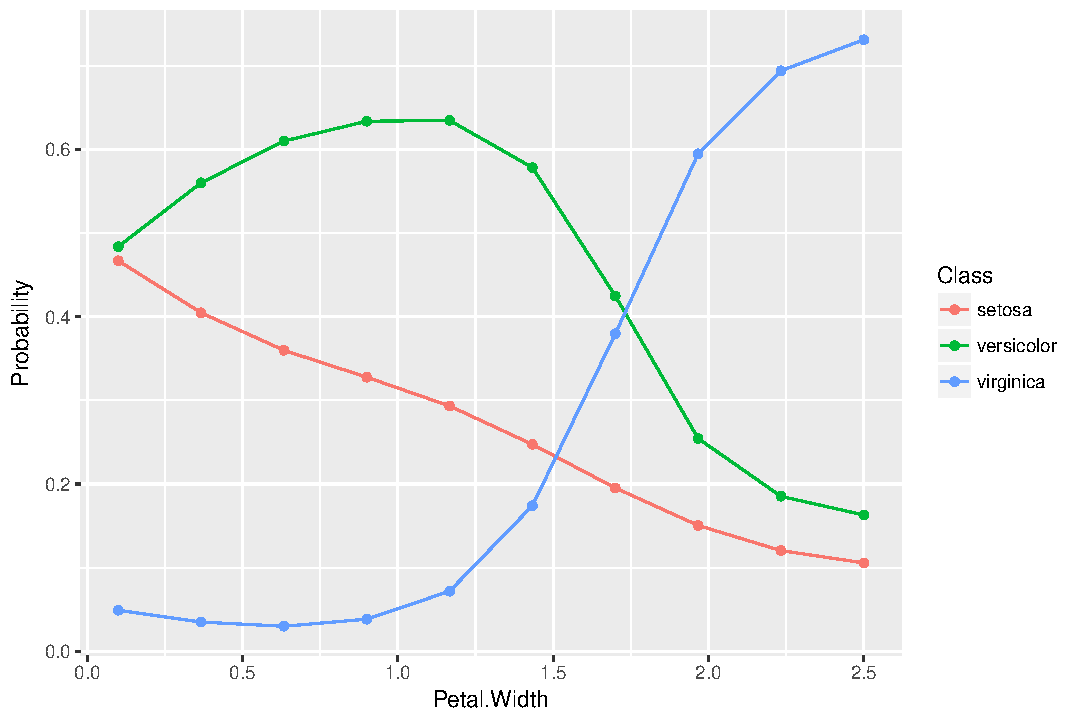
\includegraphics[width=\maxwidth]{knitr/figures/unnamed-chunk-7-1} 

}



\end{knitrout}

\noindent %' \framebreak
%' <<fig.height=4, fig.width=8>>=
%' pd = generatePartialPredictionData(fit.classif, iris.task, 
%'   "Petal.Length", individual = TRUE)
%' plotPartialPrediction(pd)
%' @
\end{vbframe}

\begin{vbframe}{\pkg{mlr} Learner Wrappers}
  \begin{blocki}{What?}
    \item Extend the functionality of learners by adding an \pkg{mlr} wrapper to them
    \item The wrapper hooks into the train and predict of the base learner and extends it
    \item This way, you can create a new \pkg{mlr} learner with extended functionality
    \item Hyperparameter definition spaces get joined!
  \end{blocki}
  \framebreak
  \begin{blocki}{Available Wrappers}
    \item \structure{Preprocessing}: PCA, normalization (z-transformation)
    \item \structure{Parameter Tuning}: grid, optim, random search, genetic algorithms, CMAES, iRace, MBO
    \item \structure{Filter}: correlation- and entropy-based, $\mathcal{X}^2$-test, mRMR, \ldots
    \item \structure{Feature Selection}: (floating) sequential forward/backward, exhaustive search, genetic algorithms, \ldots
    \item \structure{Impute}: dummy variables, imputations with mean, median, min, max, empirical distribution or other learners
    \item \structure{Bagging} to fuse learners on bootstraped samples
    \item \structure{Stacking} to combine models in heterogenous ensembles
    \item \structure{Over- and Undersampling} for unbalanced classification
  \end{blocki}
\end{vbframe}
% \begin{vframe}{Nested Resampling}
%   \begin{itemize}
%     \item Using the TuningWrapper or FeatureSelectionWrapper allows to enable nested resampling
%     \item Ensures \textbf{unbiased} results for model optimization
%     \item Everything else is statistically unsound
%   \end{itemize}
%   \begin{center}
%     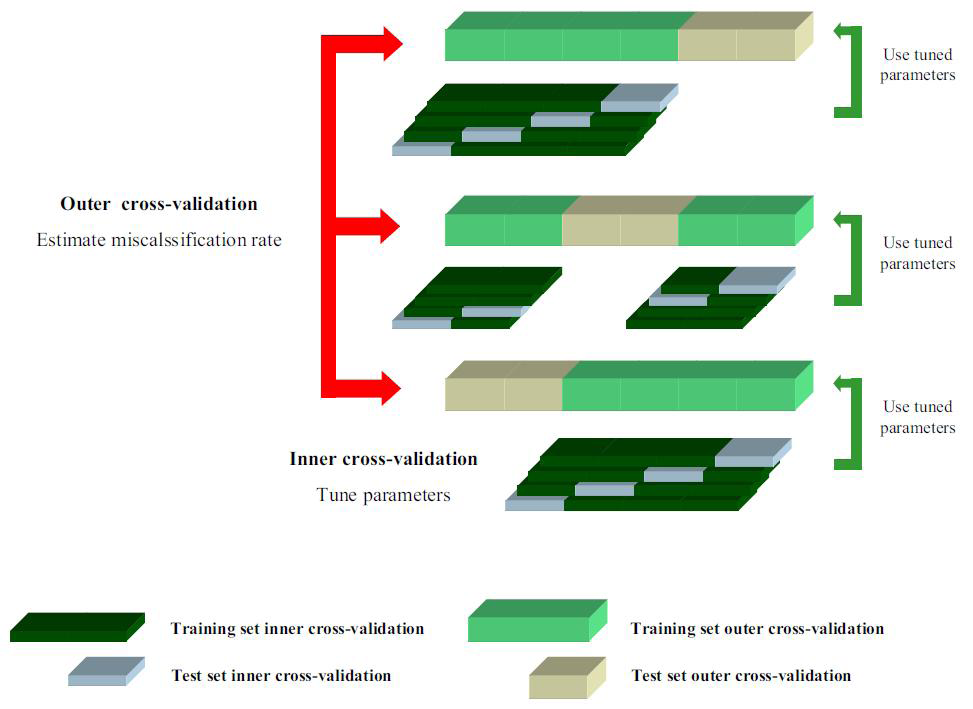
\includegraphics[width=8cm]{figure/nested.png}
%   \end{center}
% \end{vframe}
% \begin{vframe}{R Example with \texttt{FilterWrapper}}
% 
% \begin{itemize}
% %\item In the following regression example we consider the BostonHousing data set. 
% \item A Learner can be fused with any wrapper, e.g. with a feature filter. 
% %Use a regression tree and determine the optimal percentage value for feature selection such that the 3-fold cross-validated MSE of the learner is minimal. 
% %\item As search strategy for tuning a grid search is used.
% \item \texttt{makeFilterWrapper} introduces the feature selection threshold \texttt{fw.perc} (selects \texttt{fw.perc*100\%} of the top scoring features) as new hyperparameter.
% \item The optimal value for \texttt{fw.perc} can be determined by grid-search.
% \end{itemize}
% 
% <<echo=c(1,4)>>=
% lrn = makeFilterWrapper(learner = "classif.lda", fw.method = "information.gain")
% w = getOption("width")
% options(width = 160)
% getParamSet(lrn)
% options(width = w)
% @
% \end{vframe}




% % \section{Part3} %----------------------------------------------------------------------------------
% \section{Visualizations}

% \begin{vframe}{Visualizations}
%   \begin{itemize}
%     % \item A brief time ago, \pkg{mlr} was pretty bare-bones here
%     \item We use \pkg{ggplot2} and interactive \pkg{ggvis} as a standard, if possible
%     \item Some plots use Viper Charts as backend (cost curves, lift charts, \ldots)
%     \item GSOC project 2015 with Zach Jones
%     \begin{itemize}
%       \item Demo plots for models in teaching
%       \item ROC curves
%       \item Threshold vs. Performance
%       \item Partial dependency plot
%       \item Learning curves
%     \end{itemize}
%   \end{itemize}
% \end{vframe}

% \begin{vframe}{R Example}
%   \oneliner{Visualizations}
% \end{vframe}

% % \section{caret vs. \pkg{mlr}}

% % \begin{vbframe}{caret vs. mlr}


% % % \oneliner{Of course we are biased :)}

% % % \begin{blocki}{Why is caret great}
% % % \item caret is an overall great package
% % % \item caret has much better visibility
% % %   (This sucks. We will work hard on changing this)
% % % \item caret has a book (I guess we won't -- soon)
% % % \item caret has a few more regression and classification learners
% % % \item caret has (rudimentary) support for time-series data\\
% % %   (\pkg{mlr} will have that soon)
% % % \end{blocki}
% % % \framebreak

% % \begin{blocki}{Why we like \pkg{mlr} more}
% % % \item \pkg{mlr} is under active development by a substantial number of people: 6 core developers, several other packages with lots of interoperability, and 3 GSOC 2015 developers
% % \item \pkg{mlr} has (in our opinion) a better OO design, class structure and infrastructure for future development and for users
% % \item This makes things combinable, extensible, predictable
% % \item More flexible parallelization with \pkg{parallelMap}, even on HPCs via \pkg{BatchJobs}
% % \item Tuning with advanced methods like \pkg{irace}
% % \item  Fusing learners with other operations like pre-processing and feature selection
% % % \item \pkg{mlr} has better infrastructure for training, evaluating, tuning, benchmarking, and visualizing learning algorithms
% % % \item \pkg{mlr} has (vastly) better unit tests (which means it is more reliable!).
% % % \item \pkg{mlr} has better software documentation
% % % \item \pkg{mlr} has a consistent style
% % \item Nested resampling (required for unbiased results)
% % \item Survival and cluster analysis
% % % \item \textbf{With more visibility, funding, and contributors it could be even more awesome}
% % \end{blocki}

% % % \framebreak

% % % \begin{blocki}{What \pkg{mlr} can do, but caret cannot}
% % % \item Blocking in resampling
% % % \item Integrated stacking (a new separate package for caret, \pkg{caretEnsemble})
% % % \item Partial predictions/dependence for any supervised method
% % % \item Cost-sensitive learning
% % % \end{blocki}
% % \end{vbframe}


% \section{OpenML} %%%%%%%%%%%%%%%%%%%%%%%%%%%%%%%%%%%%%%%%%%%%%%%%%%%%%%%%%%%%%%%%%%%%%%%%%%%%%%%%%%%%

\begin{vframe}{OpenML}
  %\oneliner{Caution: Work in progress}
  Main idea: Make ML experiments reproducible, computer-readable and allow collaboration with others.
  %\begin{blocki}{OpenML?}
  %\item Main idea: Make ML experiments reproducible, computer-readable and allow collaboration with others.
  %\item Share everything (e.g. data sets, algorithms and results)
  %\item Enrich with meta-information
  %\item Later: Mine the results, meta-learn on it
  %\end{blocki}
  \begin{center} 
  \includegraphics[page=16,width=0.8\textwidth, height=0.7\textheight]{figure/oml-talk.pdf}
  \end{center}
\end{vframe}

\begin{vbframe}{OpenML R-Package}
  %\oneliner{Let's visit website and project page}
  %\framebreak
  \oneliner{\url{https://github.com/openml/r}}
  
  \begin{blocki}{Tutorial}
    \item \url{http://openml.github.io/openml-r}
    \item Caution: Work in progress
  \end{blocki}
  
  \begin{blocki}{Current API in R}
    \item Explore and Download data and tasks
    \item Register learners and upload runs
    \item Explore your own and other people's results
  \end{blocki}

% \framebreak
% 
% <<echo=FALSE, results='hide'>>=
% set.seed(12)
% @
% 
% <<openml1, message=FALSE>>=
% library(OpenML)
% # set apikey after install (here public read-only key)
% setOMLConfig(apikey = "c1994bdb7ecb3c6f3c8f3b35f4b47f1f", arff.reader = "RWeka")
% oml.task = getOMLTask(1)
% res1 = runTaskMlr(oml.task, makeLearner("classif.rpart"))
% res2 = runTaskMlr(oml.task, makeLearner("classif.randomForest"))
% bmr = mergeBenchmarkResultLearner(res1$bmr, res2$bmr)
% @
% 
% \framebreak
% 
% <<fig.height=4>>=
% plotBMRBoxplots(bmr)
% @

\end{vbframe}


\begin{vframe}{There is more \ldots}
  \begin{blocki*}
  \item Clustering and Survival analysis
  \item Regular cost-sensitive learning (class-specific costs)
  \item Cost-sensitive learning (example-dependent costs)
  \item ROC and learning curves
  \item Imbalancy correction
  \item Multi-Label learning
  \item Bayesian optimization
  \item Multi-criteria optimization
  \item Ensembles, generic bagging and stacking
  \item Some interactive plots with \texttt{ggvis}
  \item \ldots
  \end{blocki*}
\end{vframe}
\begin{vframe}{Outlook}
  \begin{blocki}{We are working on}
  \item Even better tuning system
  \item More interactive and 3D plots
  \item Large-Scale learning on databases
  \item Keeping the data on hard disk \& distributed storage
  \item Time-Series tasks
  \item Large-Scale usage of OpenML
  \item \texttt{auto-mlr}
  \item \ldots
  \end{blocki}
\end{vframe}
\begin{vframe}
  \oneliner{Thanks!}
\end{vframe}

\end{document}
% vim: set spelllang=en :
